%==============================================================================
\chapter{A CCM Overview}
%==============================================================================
\begin{flushright}
{\it }
\end{flushright}

%==============================================================================
\section{Introduction}
%==============================================================================

The {\it Object Management Group} (OMG) has been standardizing an open
middleware specification to support distributed applications. The OMG specified
a sophisticated component model based on the OMG's {\it Common Object Request
Broker Architecture} (CORBA). This model is called the {\it CORBA Component
Model} (CCM) \cite{CCMSpecification}.

%==============================================================================
\section{Component model}
%==============================================================================

The CCM defines a component architecture and a container framework in which the
component life cycle takes place. Components and their supporting objects
(homes, interfaces, etc.) are all defined using a formal language called the
Interface Definition Language (IDL). The CCM is part of the OMG's CORBA version
3.0 standard, so CCM descriptions use IDL3 as a specification language.

\begin{figure}[!htb]
    \begin{center}
        \includegraphics [width=6cm,angle=0] {Component}
        \caption{CCM component}
        \label{component}
    \end{center}
\end{figure}

A {\it CCM Component} (Fig.~\ref{component}) provides a variety of surface
features that support ways to connect components together to form assemblies:

\begin{description}
\item [Home]
The component {\it home} is an interface that defines factory and finder methods
to create or find component instances that the home manages. Each home supports
at least one {\tt create} method.

\item [Equivalent interface]
Every IDL3 interface (containing the keywords {\tt component}, {\tt home}, etc.)
can be transformed into a classic IDL interface, one that can be processed by a
regular IDL compiler. This classic IDL interface is known as the {\it equivalent
interface\/}. The IDL3 to IDL mapping adds some interfaces and equivalent
operations to the interfaces specified by the user in the IDL3 source file. As
described by the CCM specification, every IDL3 construct defines its own IDL3 to
IDL mapping.

\item [Supported interface]
A home or component definition can {\it support} zero or more interfaces. Each
supported interface results in an inheritance of supported interfaces in the
corresponding equivalent interfaces. Supported interfaces basically give
component designers a way to assign context--free methods to a component.

\item [Attribute]
A component or a component home can have {\it attributes\/}. Attributes are
named values exposed through accessor and mutator operations (otherwise known as
get and set operations). Attributes are primarily intended to be used for
component configuration.

\item [Facet]
A component {\it facet} is a named interface that provides access to specific
component methods. A component may have zero or more facets. The component's
equivalent interface inherits the {\tt Components::Navigation} interface; this
interface defines generic operations for facet access. Facets can be seen as a
way for component designers to assign contextual methods to a component; that
is, the methods defined in a facet interface can only be called if the component
has one or more compatible receptacles attached to the facet.

\item [Receptacle]
A component {\it receptacle} is an abstract way of creating a socket on a
component that receives connections of a certain type. Thus receptacles are
concretely manifested on a component as a set of operations for establishing and
managing connections. A component may have zero ore more receptacles. The
component's equivalent interface inherits the {\tt Components::Receptacles}
interface; this interface defines generic operations for receptacle management.
Like facets, the operations defined in a receptacle interface can be seen as
contextual methods; they require a connected facet to function correctly.

\item [Event source]
An {\it event source} embodies the potential for the component to generate
events of a specified type and provides mechanisms for associating consumers
with sources. There are two categories of event sources, {\it emitters} and {\it
publishers}. An emitter can be connected to at most one proxy provider by the
container. A publisher can be connected through the channel to an arbitrary
number of consumers that are subscribed to the publisher event source.

\item [Event sink]
An {\it event sink} embodies the potential for the component to receive events
of a specified type.
\end{description}

The component model is also defined in a MOF compliant metamodel, the {\it
Interface Repository Metamodel}. The Interface Repository Metamodel expresses
the extensions to classic IDL defined by the CCM.

%==============================================================================
\section{Component container}
%==============================================================================

Components run in a {\it CCM Container} (Fig.~\ref{container}). Containers
provide the runtime environment for CORBA components. Containers are built on
the {\it Object Request Broker} (ORB), the {\it Portable Object Adapter} (POA),
and other CORBA services.

\begin{figure}[!htb]
    \begin{center}
        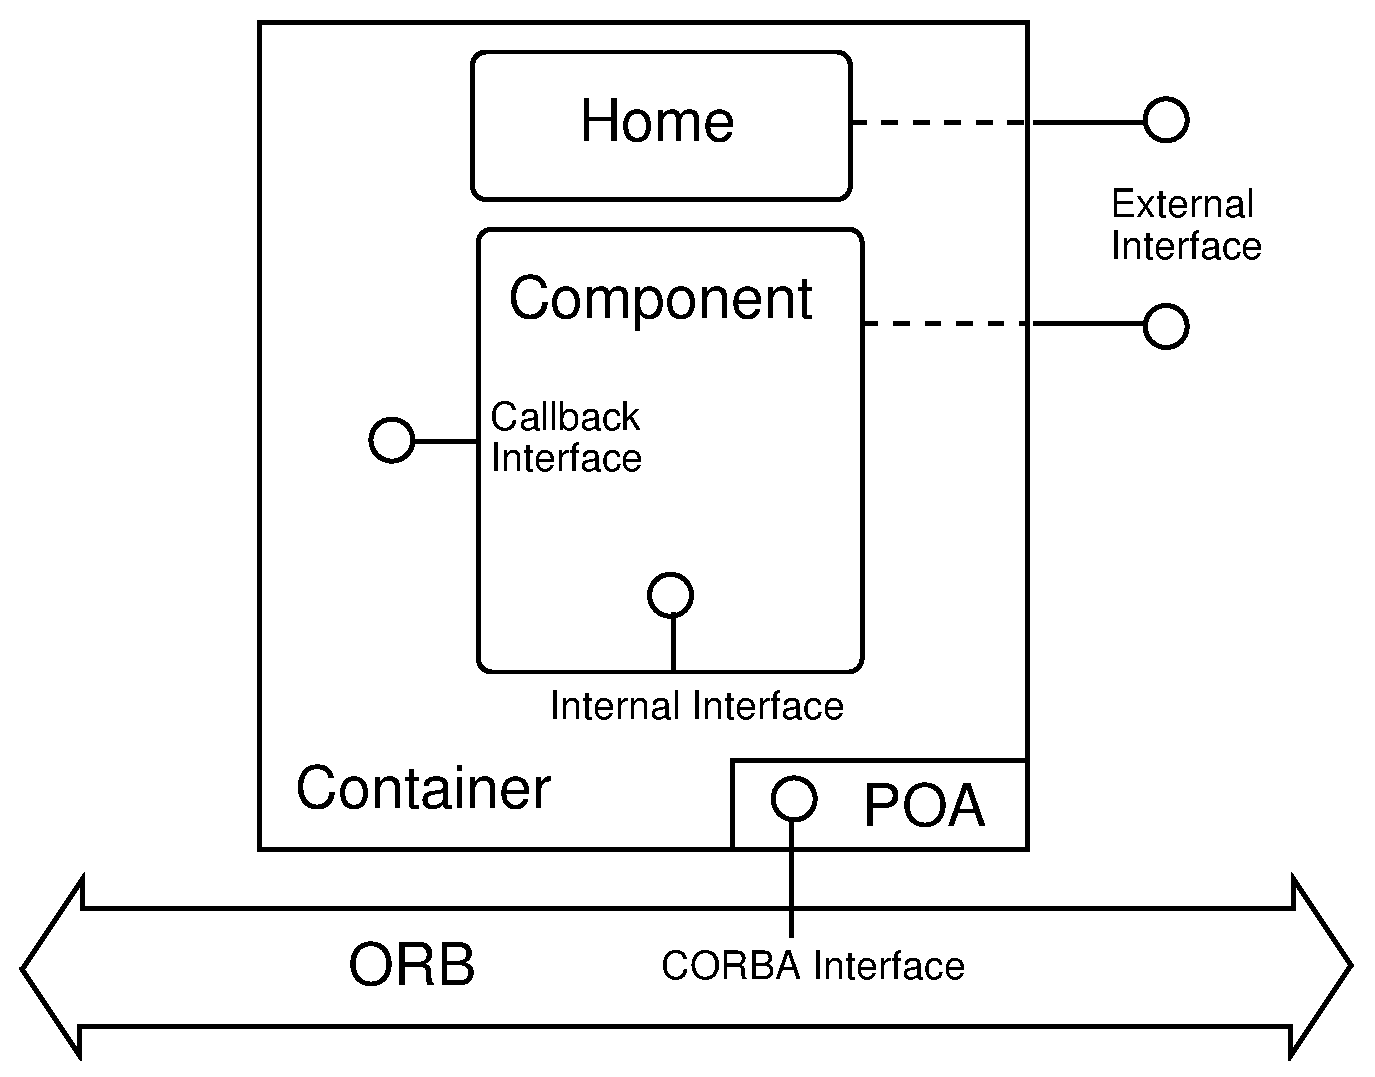
\includegraphics [width=6cm,angle=0] {Container}
        \caption{CCM container}
        \label{container}
    \end{center}
\end{figure}

As shown in Fig.~\ref{container}, the container programming model is made of
interfaces that are used by the client, the container, and the components. These
interfaces fall into the following three categories:

\begin{description}
\item [Internal interfaces]
These local interfaces are used by the component developer and provided by the
container to assist in the implementation of the component's behavior.

\item [External interfaces]
The external interfaces define the external view of a component. They are used
by the client and implemented by the component developer.

\item [Callback interfaces]
These local interfaces are used by the container and implemented by the
component, either in generated code or directly, so that the component can be
deployed in the container.
\end{description}

The CCM specification defines four component categories. The behavior of these
categories is specified by the container interface types. Additionally, there is
a component category that describes the empty container.

\begin{description}
\item [Service component]
The {\it service component} has behavior, no state, and no identity. The
lifespan of a service component is equivalent to the lifetime of a single
operation request.

\item [Session component]
The {\it session component} has behavior, transient state, and an identity
(which is not persistent). Note that the session component is equivalent to the
stateful session bean found in Enterprise Java Beans (EJB).

\item [Process component]
The {\it process component} has behavior, persistent state (which is not visible
to the client), and a persistent identity.

\item [Entity component]
The {\it entity component} has behavior, persistent state (which is visible to
the client), and an identity (which is visible to the clients through a primary
key declaration).
\end{description}

%==============================================================================
\section{Component assembly}
%==============================================================================

Often in practice components are not large enough to safely encapsulate the
operations and data necessary for complex processes. The CCM specification
provides a way to form component {\it Assemblies} (Fig.~\ref{assemblygraph}) by
connecting components through their facets and receptacles.

\begin{figure}[!htb]
    \begin{center}
        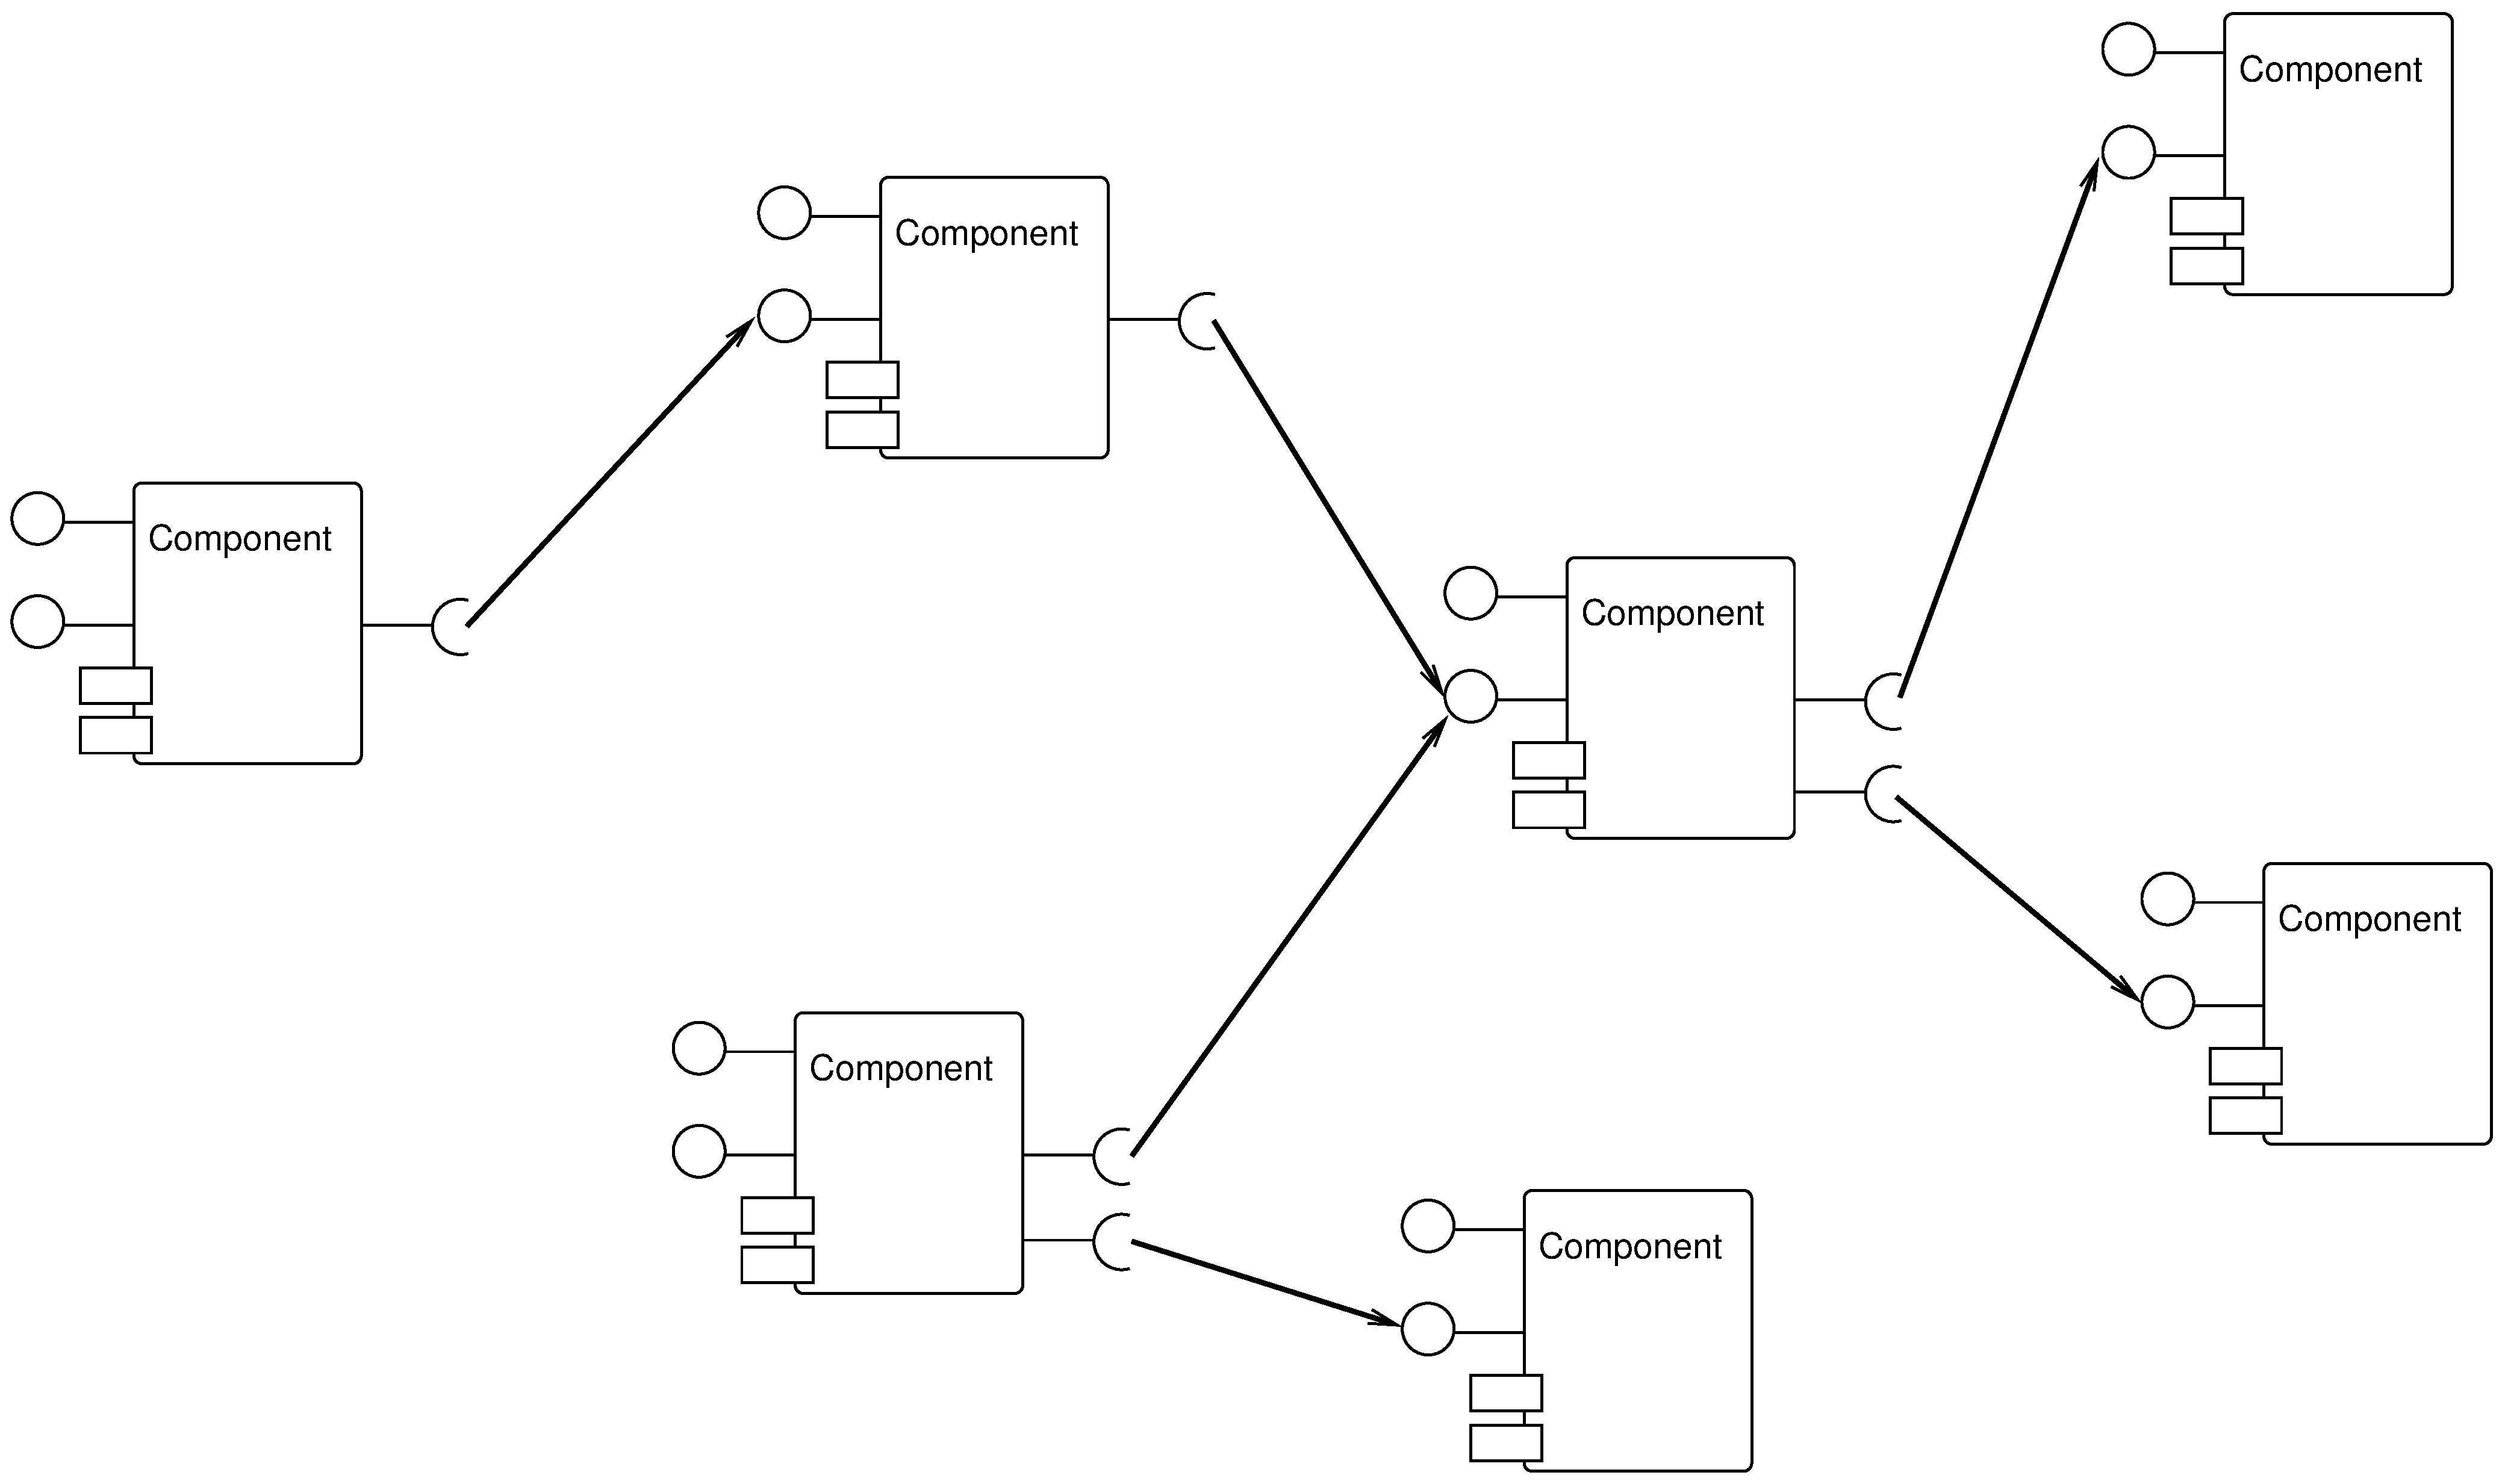
\includegraphics [width=6cm,angle=0] {Assembly}
        \caption{Component assembly}
        \label{assemblygraph}
    \end{center}
\end{figure}

The CCM specification also defines a {\tt Components::Assembly} interface that
represents an assembly instance. It is used to build up and tear down component
assemblies. Building the assembly up means creating all of the necessary
components and establishing connections between them as specified in a file
called the {\it assembly descriptor\/}. Tearing the assembly down means removing
all connections and destroying the components.

%==============================================================================
\section{Descriptor files}
%==============================================================================

The CCM specification defines the formats of several XML descriptor files that
are used to describe software packages, components, properties, and assemblies.

\begin{description}
\item [Software package descriptor (*.csd)]
The software package descriptor consists of general information about the
software followed by one or more sections describing implementations of
software.

\item [CORBA component descriptor (*.ccd)]
The component descriptor specifies component characteristics that a design tool
might use to display information about a component (e.g. supported interfaces,
inherited components, used and provided ports, etc.).

\item [Component assembly descriptor (*.cad)]
The assembly descriptor consists of elements describing the components used in
an assembly, connection information, and partitioning information.

\item [Property file descriptor (*.cpf)]
The property file is used at deployment time to configure a home or a component
instance. A configurator uses the property file to determine how to set
component and home property attributes.
\end{description}

%==============================================================================
\section{Client programming model}
%==============================================================================

The client interacts with a CORBA component through two forms of external
interfaces, a home interface and one or more application interfaces. Two forms
of clients are supported by the CCM specification:

\begin{description}
\item [Component--aware client]
This client knows that it is making requests to a component. The client can use
component mechanisms like navigation between components through facets and
receptacles, etc. Component--aware clients locate their interfaces using the
{\tt Components::HomeFinder} or a naming service.

A reference that supports the {\tt HomeFinder} interface may be obtained from
the ORB by invoking {\tt CORBA::ORB::resolve\_initial\_references()} with the
parameter value {\tt ``ComponentHomeFinder''}.

\item [Component--unaware client]
This client does not know that there is a CORBA component. The client requests
are made as if the requests are going to ordinary CORBA objects and object
factories.
\end{description}
